\documentclass[12pt]{article}
\usepackage{graphicx}

\newcommand{\WZ}{\ensuremath{\mathrm{W}\mathrm{Z}}}
\newcommand{\WW}{\ensuremath{\mathrm{W}^\pm\mathrm{W}^\pm}}
\newcommand{\jet}{\ensuremath{\mathrm{j}}}
\newcommand{\mjj}{\ensuremath{m_{\jet\jet}}}
\begin{document}

\title{Probing the Standard Model with a boson-boson collider}
\date{\today}
\maketitle

The weak force is one of the four fundamental interactions between elementary particles, along with the electromagnetic, strong, and gravitational forces, and is responsible for the radioactive decay. The weak force carriers are the heavy $\mathrm{W}^{\pm}$, $\mathrm{W}^{-}$, and Z bosons, about 80 to 90 times heavier than the proton; first confirmed with the Super Proton Synchroton accelerator at CERN in 1983. The Standard Model (SM) of particle physics predicts self interactions between these heavy bosons. Studies of these self interactions, known as triple- and quartic-gauge-couplings, provide key insight into the structure of the SM and can reveal hints of contributions from yet unknown physics. 

Can we build a heavy W and Z boson collider in the tunnel of the Large Hadron Collider (LHC) to study their self interactions? At first glance this is impossible as the W and Z bosons have extremely short lifetimes and travel only distances of about $0.1 \times 10^{-15}$ meters before decaying to other particles and can't be used as targets or projectiles; or can they? During rare occasions a W or Z boson is created inside a proton and even more rarely this happens inside two colliding protons at the LHC resulting in unlikely collisions of two bosons as illustrated with a so called Feynman diagram in Figure~\ref{fig:feynman}. There are approximately 1 billion proton-proton collisions per second at the LHC and these extremely rare vector boson scattering (VBS) events are recorded once every 1000 billion proton-proton collisions.

\begin{figure*}[htb]
\centering
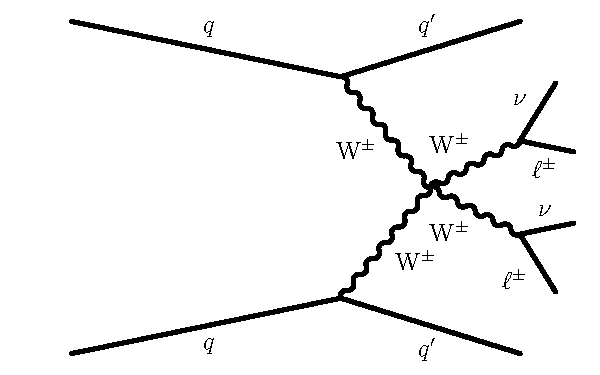
\includegraphics[width=0.60\textwidth]{figures/leptonic_vbs_quartic.pdf}
\caption{An example Feynman diagram: two quarks from the incoming protons come from the left and produce two W bosons that self interact in the center (so called quartic-gauge-vertex). The outgoing W bosons decay into a charged lepton (electron or muon) and the corresponding neutrino. On the right there are also two quarks remaining that tend to point along the direction of the LHC beam.}
\label{fig:feynman}
\end{figure*}

The discovery of a Higgs boson by both the ATLAS and CMS experiments in 2012 confirmed the electroweak symmetry breaking mechanism, the process through which elementary particles, including the W and Z bosons, gain mass via interaction with the Brout-Englert-Higgs field.  In fact, the LHC was built with a guaranteed discovery: we would either find a Higgs boson or discover new physics in VBS at high energies. This is due to the fact that if we calculate the amplitude of the triple-gauge-boson and quartic-gauge-boson interactions the theory runs into trouble at high energies predicting probabilities of collisions larger than 1. Only after the inclusion of the Higgs boson in the theory the predictions make sense. Thus, the study of the VBS process provides a treasure trove of information on the heavy boson self interactions as well as the electroweak symmetry breaking mechanism.

%interaction (Figure~\ref{fig:feynman}, left)  we find that the amplitude grows with center of mass energy (E) with $E^4$ behavior. This means that the theory runs into trouble at high energies as the probability can not be bigger than 1. The inclusion of the quartic-gauge-coupling diagram (Figure~\ref{fig:feynman}, center) cancels the undesired $E^4$ behavior but a part behaving as $E^2$ remains. 

Using the data collected during 2016-18 CMS has performed detailed studies of the production of the same-sign $\WW$ and $\WZ$ boson pairs using the leptonic decays (electrons and muons). The VBS final states at the LHC have a striking signature  with two jets (originating from the two initial quarks that initially radiated the W or Z bosons) in the opposite hemispheres of the CMS detector closer to the LHC beamline and with a large invariant mass ($\mjj$) as shown in Figures xx and yy (event displays). The $\WW$ and $\WZ$ production modes are studied together by simultaneously measuring them using several kinematic observables.  

The CMS collaboration had reported the first observation of the EW  $\WW$ production at 13 TeV with significance greater than 5 standard deviation using the data collected in 2016. Results close to 5.0 standard deviations indicate a one in a million chance of the result arising from a statistical fluctuation. First detailed studies of the $\WW$ production as functions of different kinematic variables are performed with this larger dataset. An excellent agreement with the SM predictions are reported as can be seen in Figure~\ref{fig:signal} (left). Machine learning is used to establish the first observation of the electroweak production of the $\WZ$ boson pairs with the CMS detector as shown in Figure~\ref{fig:signal} (right). The observed statistical significance is 6.8 standard deviations with 5.3 standard deviations expected from the SM predictions. Strong constraints on anomalous quartic-gauge-couplings are also set using the $\WW$ and $\WZ$ final states. 

\begin{figure*}[htb]
\centering
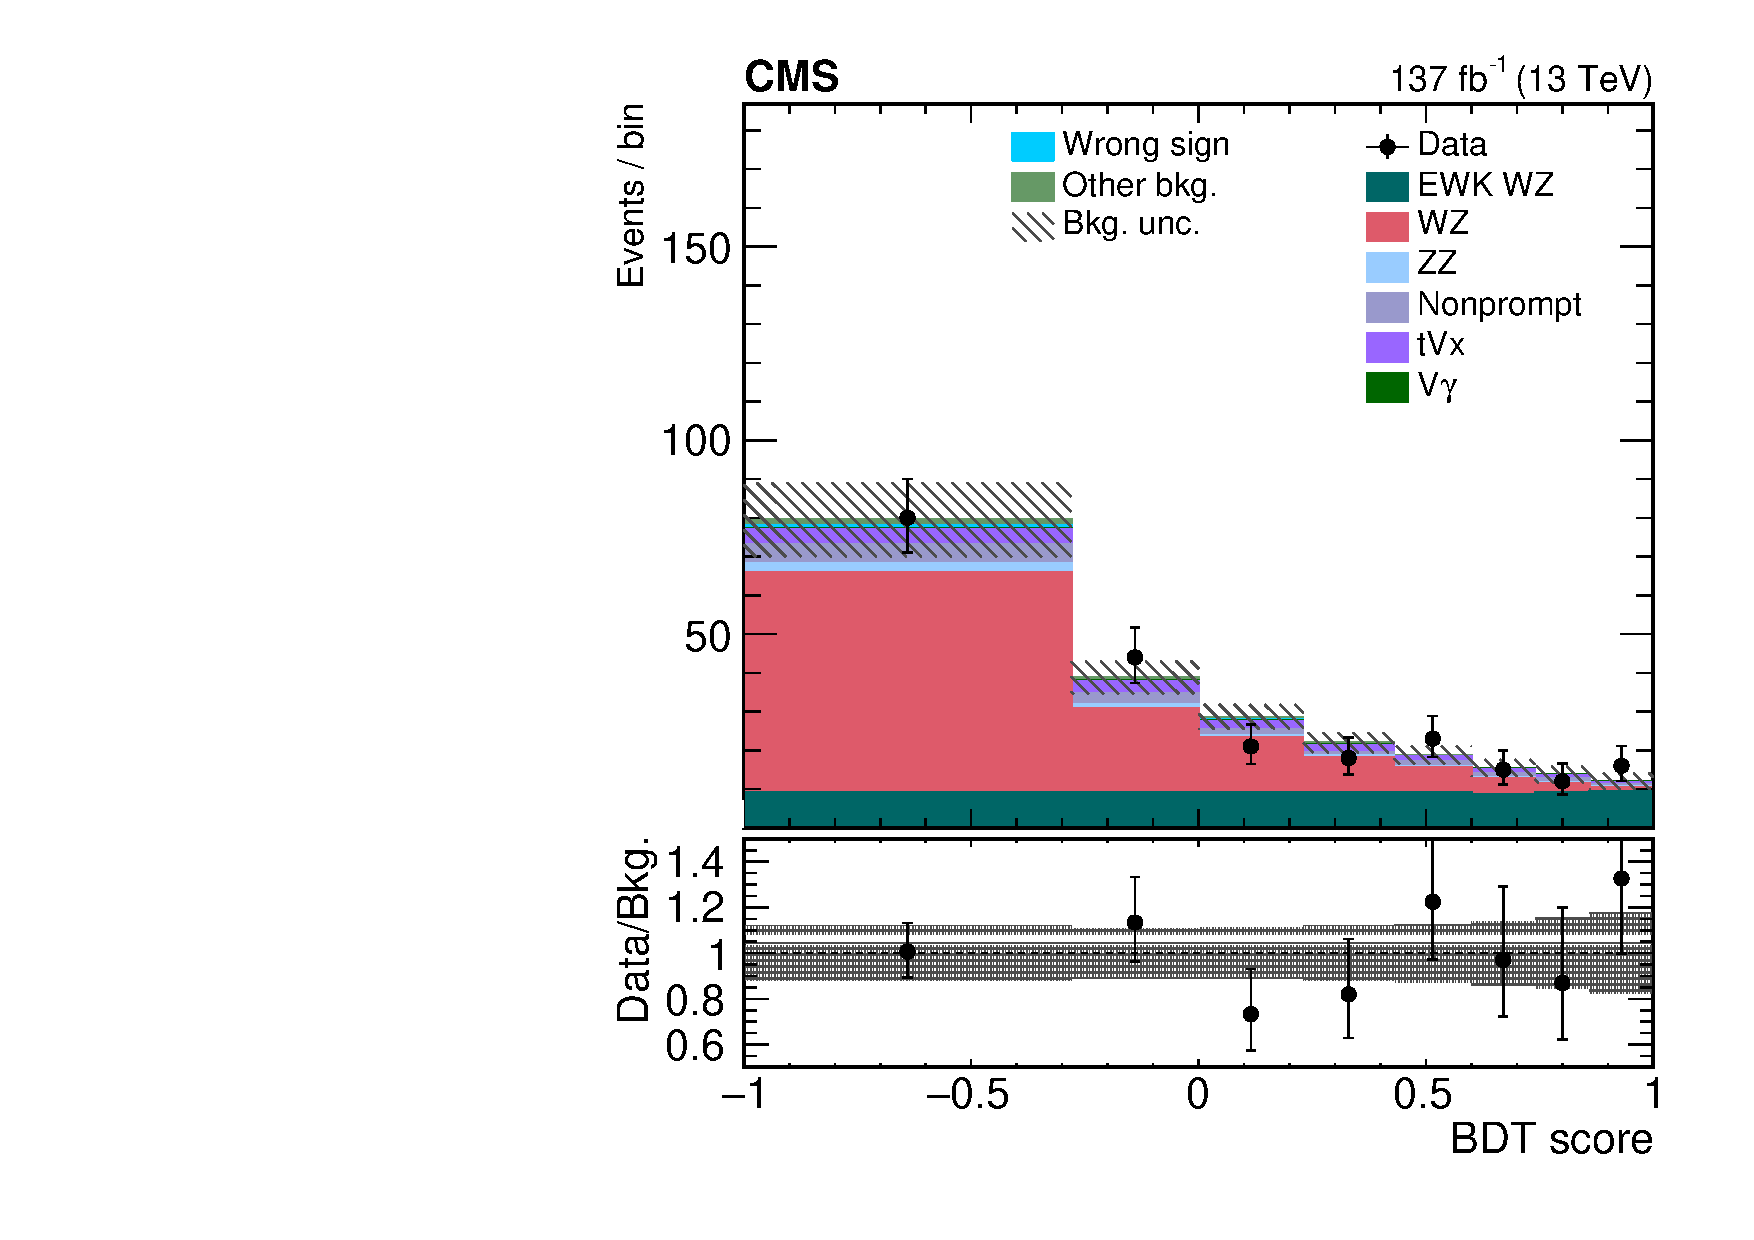
\includegraphics[width=0.49\textwidth]{figures/ssww_wzsel_bdt_2019.pdf}
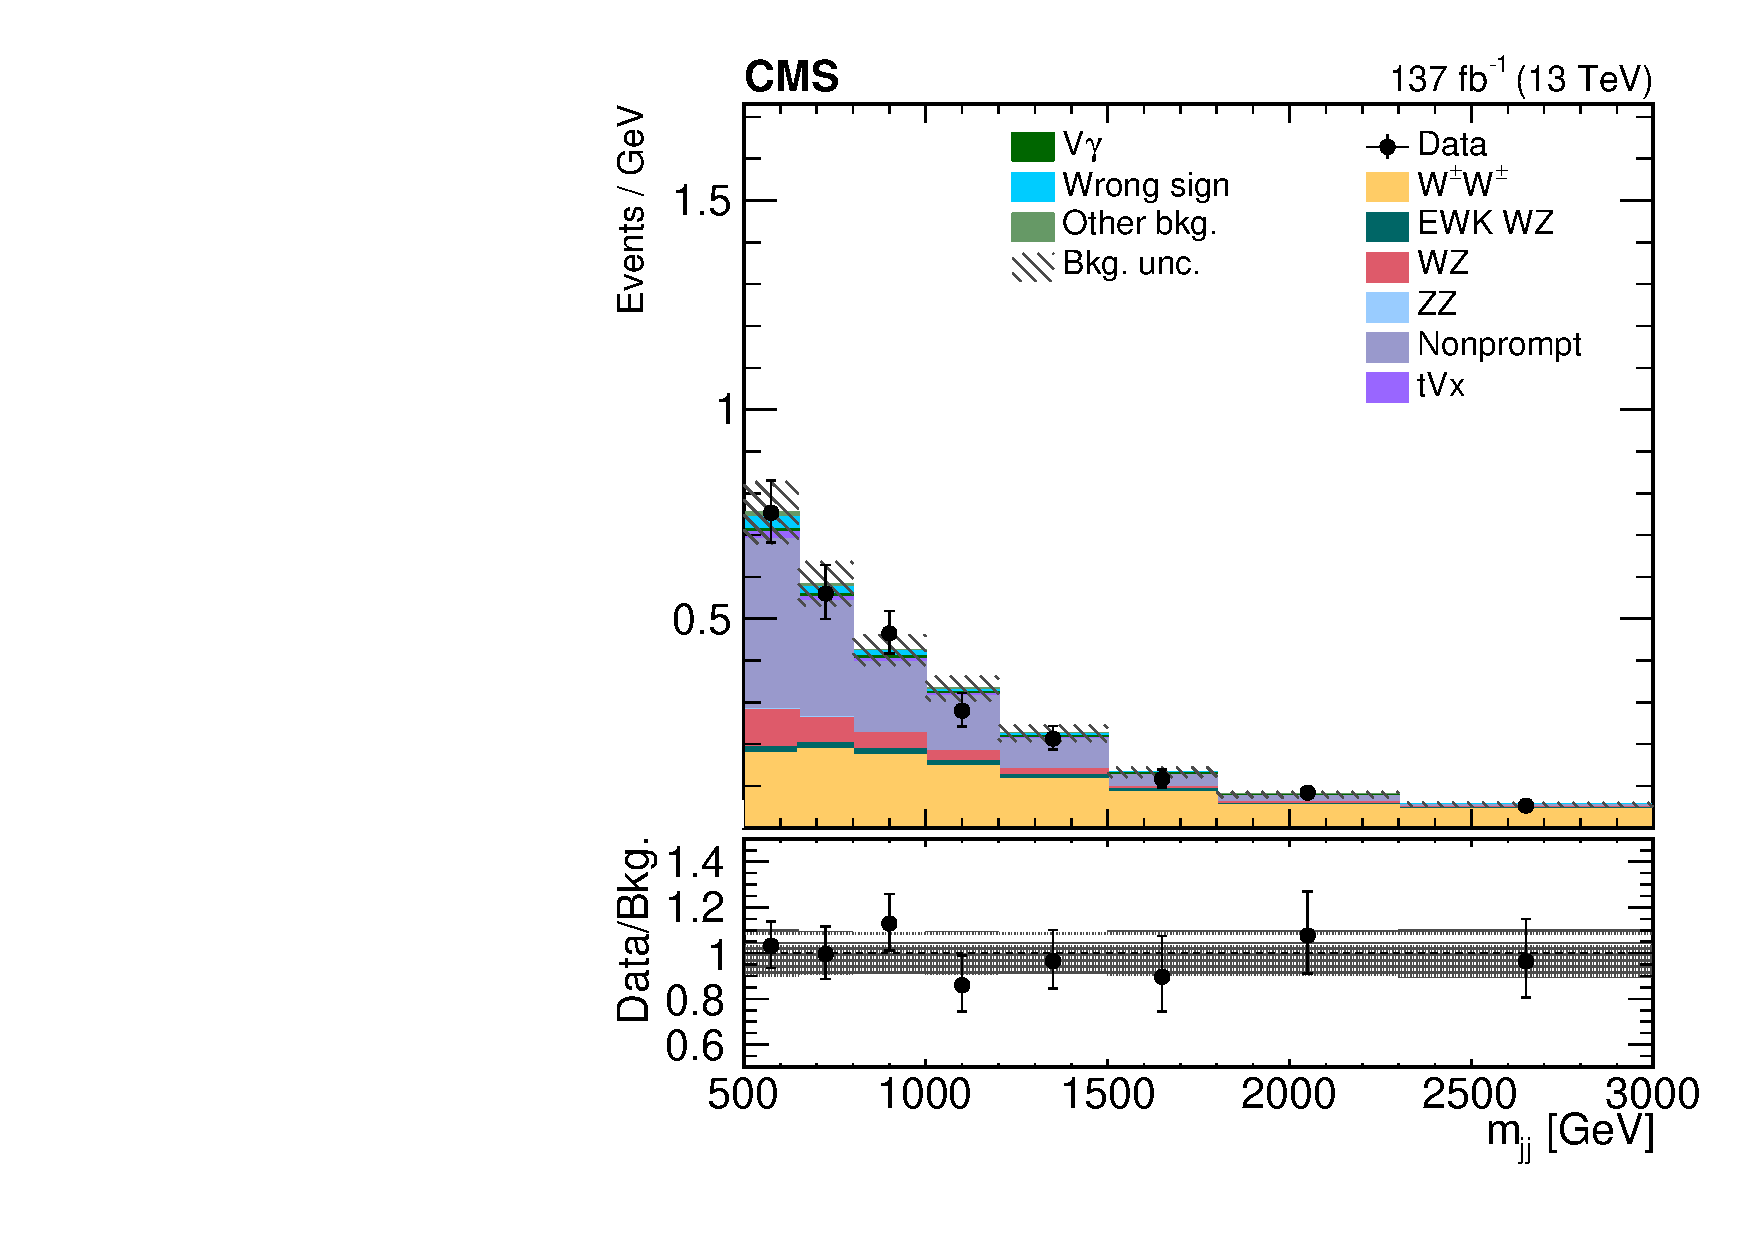
\includegraphics[width=0.49\textwidth]{figures/ssww_wwsel_mjj_2019.pdf}
\caption{Distributions of $\mjj$ in the $\WW$ signal region (left) and  BDT score in the $\WZ$ signal region. The bottom panel in each figure
shows the ratio of the number of events observed in data to that of the total SM prediction.
The gray bands represent the uncertainties from the predicted yields.}
\label{fig:signal}
\end{figure*}

The observations of the  electroweak production of $\WW$ and $\WZ$  boson pairs are important milestones towards precision tests of VBS at the LHC, and there is much more to be learned from the LHC Run 3 data. Models of physics beyond the SM predict enhancements to VBS via modifications to the Higgs sector, or from the presence of additional resonances. Studies demonstrate that the High Luminosity LHC, due to enter operation in the middle 2020s, should allow very precise investigations of W-boson scattering with great sensitivity to the electroweak symmetry breaking mechanism.

\end{document}

